\RequirePackage[l2tabu,orthodox]{nag} % turn on warnings because of bad style
\documentclass[a4paper,11pt,bibtotoc]{scrartcl}

\usepackage[utf8]{inputenc}     % This allows to type UTF-8 characters like ä,ö,ü,ß

\usepackage[T1]{fontenc}        % Tries to use Postscript Type 1 Fonts for better rendering
\usepackage{lmodern}            % Provides the Latin Modern Font which offers more glyphs than the default Computer Modern
\usepackage[intlimits]{amsmath} % Provides all mathematical commands

\usepackage{hyperref}           % Provides clickable links in the PDF-document for \ref
\usepackage{grffile}            % Allow you to include images (like graphicx). Usage: \includegraphics{path/to/file}

% Allows to set units
\usepackage{siunitx}
\sisetup{per-mode=fraction}     % Optional

% Additional packages
\usepackage{url}                % Lets you typeset urls. Usage: \url{http://...}
\usepackage{breakurl}           % Enables linebreaks for urls
\usepackage{xspace}             % Use \xpsace in macros to automatically insert space based on context. Usage: \newcommand{\es}{ESPResSo\xspace}
\usepackage{xcolor}             % Obviously colors. Usage: \color{red} Red text
\usepackage{booktabs}           % Nice rules for tables. Usage \begin{tabular}\toprule ... \midrule ... \bottomrule

% Source code listings
\usepackage{listings}           % Source Code Listings. Usage: \begin{lstlisting}...\end{lstlisting}

\definecolor{codegreen}{rgb}{0,0.6,0}
\definecolor{codegray}{rgb}{0.5,0.5,0.5}
\definecolor{codepurple}{rgb}{0.58,0,0.82}
\definecolor{backcolour}{rgb}{0.95,0.95,0.92}

\lstdefinestyle{mystyle}{
	backgroundcolor=\color{backcolour},   
	commentstyle=\color{codegreen},
	keywordstyle=\color{magenta},
	numberstyle=\tiny\color{codegray},
	stringstyle=\color{codepurple},
	basicstyle=\ttfamily\footnotesize,
	breakatwhitespace=false,         
	breaklines=true,                 
	captionpos=b,                    
	keepspaces=true,                 
	numbers=left,                    
	numbersep=5pt,                  
	showspaces=false,                
	showstringspaces=false,
	showtabs=false,                  
	tabsize=2
}

\lstset{style=mystyle}

\begin{document}

\titlehead{Simulation Methods in Physics I \hfill WS 2021/2022}
\title{First exercise sheet in Simulation Methods in Physics I}
\author{Cedric Förch, Niklas Abraham}
\date{\today}
\publishers{Institute for Computational Physics, University of
  Stuttgart}
\maketitle

\tableofcontents

\section{Exercise 2.1}

In the first exercise we calculated the trajectory of a canonball in the air, without air resistance.
The task was to test this with a couple of different initial masses. The results are shown in the follwoing diagram:
% file is in the same folder as this file, name is ex_1.png
\begin{figure}[!htbp]
	\centering
	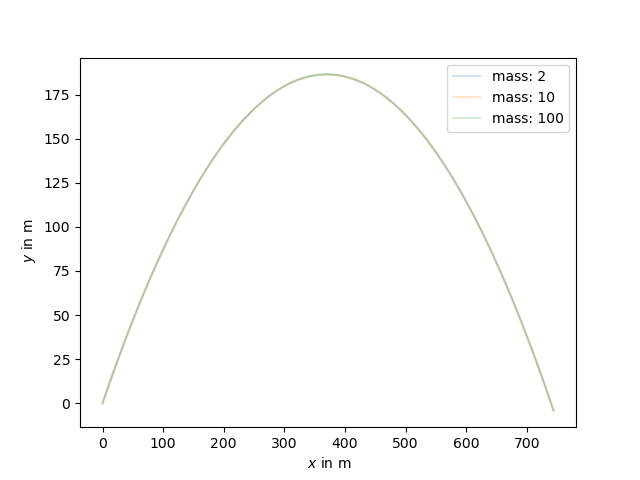
\includegraphics[width=0.6\textwidth]{ex_1.png}
	\caption{Trajectory of a canonball with different masses}
	\label{fig:ex_1}
\end{figure}
\\


\section{Exercise 2.2}

Here we created the diagram with various fricition and wind settings. We used the following settings: first without fricition and wind, then without wind but with friction and last with fricition and wind speeds of -30m/s.
The results are shown in the following diagram:
% file is in the same folder as this file, name is ex_2_2.png
\begin{figure}[!htbp]
	\centering
	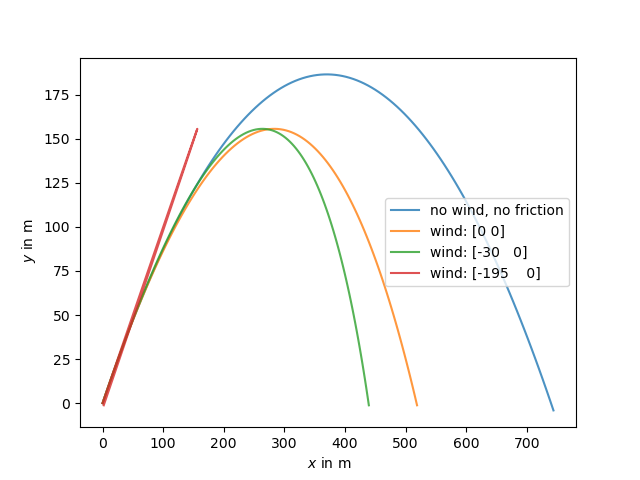
\includegraphics[width=0.6\textwidth]{ex_2_1.png}
	\caption{Trajectory of a canonball with different fricition and wind settings}
	\label{fig:ex_2_2}
\end{figure}

The wind speed for which the canonball reaches the starting point is roughly $v_{wind} = -195m/s$.

\section{Exercise 3.1}

In the third exercise we calculated the trajectory of various particles with gravitional forces.
The plot of the trajectories is shown in the following diagram:
% ex_3_1_1.png is in the same folder as this file
\begin{figure}[!htbp]
	\centering
	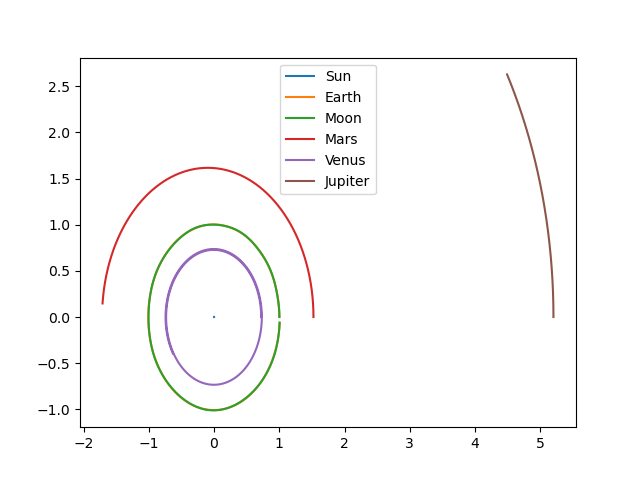
\includegraphics[width=0.6\textwidth]{ex_3_1_1.png}
	\caption{Trajectory of various particles with gravitional forces}
	\label{fig:ex_3_1_1}
\end{figure}


The difference in timestep size between 0.001 and 0.0001 are shown in the resting frame of the moon and earth. The results are shown in the following diagram:
% ex_3_1_2.png is in the same folder as this file
\begin{figure}[!htbp]
	\centering
	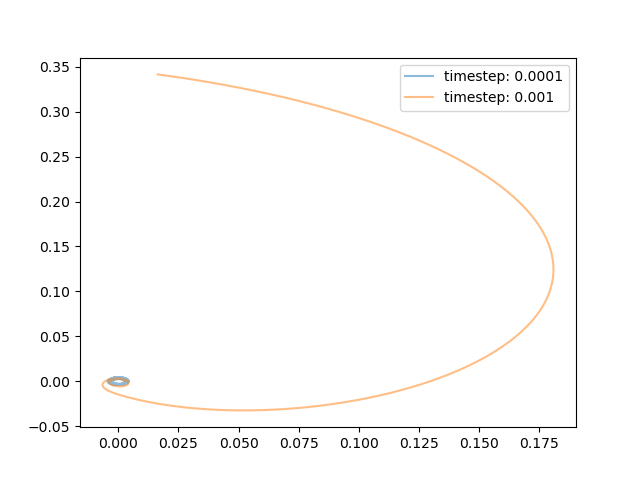
\includegraphics[width=0.6\textwidth]{ex_3_1_2.png}
	\caption{Trajectory of particles with different timestep sizes}
	\label{fig:ex_3_1_2}
\end{figure}


The part using the most time in the simulation is the calculation of the forces between the particles. Since there are two nested loops, the time complexity is $O(n^2)$.
This could be reduced by using smart saving of results, but still would consume the most time in this code.

\section{Exercise 3.2}

We start with the Taylor expansion of $x(t + \Delta t)$:
\begin{align}
	x(t + \Delta t) &= x(t) + v(t) \Delta t + \frac{1}{2} a(t) \Delta t^2 + O(\Delta t^3)
\end{align}
That is the position update of the Verlet algorithm.

For the velocity Verlet algorithm we need to expand $v(t + \Delta t)$:
\begin{align}
	v(t + \Delta t) &= v(t) + a(t) \Delta t + \frac{1}{2} \frac{d^2 v(t)}{dt^2} \Delta t^2 + O(\Delta t^3)
\end{align}

We now need to expand $\frac{d^2 v(t)}{dt^2}$ to the first order:
\begin{align}
	\frac{d^2 v(t)}{dt^2} &= \frac{d}{dt} a(t) = \frac{a(t + \Delta t) - a(t)}{\Delta t} + O(\Delta t)
\end{align}

Combined this results in the velocity Verlet algorithm:
\begin{align}
	x(t + \Delta t) &= x(t) + v(t) \Delta t + \frac{1}{2} a(t) \Delta t^2 \\
	v(t + \Delta t) &= v(t) + \frac{1}{2} (a(t) + a(t + \Delta t)) \Delta t 
\end{align}	

Now we rearrange the velocity Verlet algorithm to show that it is equivalent to the standard Verlet algorithm:
\begin{align}
	x(t + \Delta t) &= x(t) + v(t) \Delta t + \frac{1}{2} a(t) \Delta t^2 \\
	v(t + \Delta t) &= v(t) + \frac{1}{2} (a(t) + a(t + \Delta t)) \Delta t
\end{align}

We can now express $a(t + \Delta t)$ using the Verlet algorithm:
\begin{align}
	a(t + \Delta t) &= \frac{f(x(t + \Delta t))}{m} \\
	&= \frac{f(x(t) + v(t) \Delta t + \frac{1}{2} a(t) \Delta t^2)}{m} \\
	&= \frac{f(x(t)) + f'(x(t)) v(t) \Delta t + \frac{1}{2} f''(x(t)) a(t) \Delta t^2}{m} + O(\Delta t^3)
\end{align}

We can now plug this into the velocity Verlet algorithm:
\begin{align}
	x(t + \Delta t) &= x(t) + v(t) \Delta t + \frac{1}{2} a(t) \Delta t^2 \\
	v(t + \Delta t) &= v(t) + \frac{1}{2} (a(t) + \frac{f(x(t)) + f'(x(t)) v(t) \Delta t + \frac{1}{2} f''(x(t)) a(t) \Delta t^2}{m}) \Delta t
\end{align}

We can now rearrange the terms to show that the velocity Verlet algorithm is equivalent to the standard Verlet algorithm:


The difficulty of the velocity Verlet algorithm is that we need to calculate the force at the new position $x(t + \Delta t)$, which is not known yet.
This makes it hard to update the position and velocity at the same time, since we need to calculate the force at the new position.

The different algorithms are compared in the following diagram, where we simulated the trajectory of all particles for one year at a timestep of 0.01 and showed moon in the resting frame of the earth.
% ex_3_2_1.png is in the same folder as this file
\begin{figure}[!htbp]
	\centering
	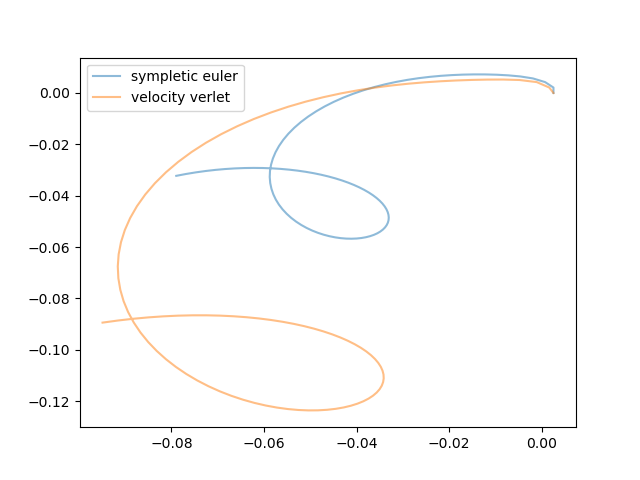
\includegraphics[width=0.6\textwidth]{ex_3_2_1.png}
	\caption{Trajectory of particles with different integrators}
	\label{fig:ex_3_2_1}
\end{figure}

\section{Exercise 3.3}

The results of the different integrators are shown in the following diagram, where we simulated the trajectory of all particles for one year at a timestep of 0.01 and showed the distance from earth to the moon over time.
The expected results is no change in distance, since the particles are in a stable orbit.

% ex_3_3_1.png is in the same folder as this file
\begin{figure}[!htbp]
	\centering
	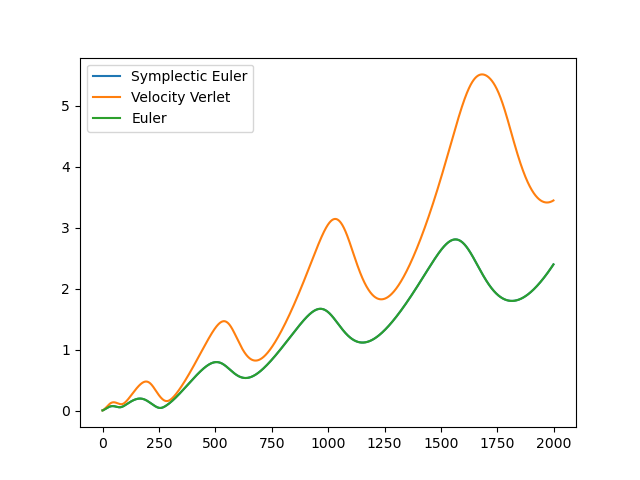
\includegraphics[width=0.6\textwidth]{ex_3_3_1.png}
	\caption{Distance from earth to moon over time}
	\label{fig:ex_3_3_1}
\end{figure}



\end{document}

